The recent observations by \citet{Lyne2010} suggest that for a few pulsars the
quasi-periodic structure observed in pulsar timing residuals is a result of 
torque-switching events. They find that the spin-down periodically switches
between two distinct values and these changes correlate with changes in the beam
width. They argue this indicates that the electromagnetic torque is periodically
switching between two distinct states. 

We will not discuss where the periodic nature comes from here, but instead
present a direct simulation of the timing residuals from switching events. For
simplicity we begin by consider a single switch in the torque at some time
$t_{\mathrm{switch}}$; for the time being we set this to be half the
observation period, such that $t_{\mathrm{switch}} = \To/2$.

In the EM dipole spindown model the torque has two distinct components: the
regular spin-down part and the so-called anomalous component. This later term 
does not contribute to the spin-down, but as discussed in section \ref{sec: effective
body frame} it will modify the axis of precession. The torque switching will 
occur in the spin-down component, but it seems unlikely that it will also
occur in the anomalous component [Ian - why?]. To cover all cases we 
model a single torque switching effect by redefining the torque in equation
\eqref{eqn: torque} such that

\newcommand{\Ss}{S_{\mathrm{S}}}
\newcommand{\Sa}{S_{\mathrm{A}}}

\begin{equation}
\mathbf{T} = (1 - \Ss H(t-t_{\mathrm{switch}})) \mathbf{T}_{\mathrm{S}}+
                 (1 - \Sa H(t-t_{\mathrm{switch}})) \mathbf{T}_{\mathrm{A}}
\label{eqn: single switch torque}
\end{equation} 
where the subscripts label the spin-down and anomalous components, $S$ is the
strength of switching, and $H(t)$ is the Heaviside function. 

Numerically solving the body-frame and Euler equations using this torque we 
simulate a single switching event to try and understand the effect it will have
on phase residuals. 

\subsubsection{Minimal precession}
Without the torque-switching, in these simulations only free precession can 
produce structure in the phase residuals. No pulsars exist with regular periodic
structure that can be solely interpreted as free precession. Most pulsars must 
therefore exist with very small wobble angles with any excitement of this being
damped. As such, we begin by discussing the "minimal precession" initial 
conditions from which to start our simulations. 


Precession will not occur when the spin vector is aligned with the axis about
which it rotates. The angle between these two we have defined as the wobble
angle.  For minimal precession we should therefore set this wobble angle to
zero. In all simulations we consider a biaxial body with the full torque given
in \eqref{eqn: single switch torque}. From our previous discussion on the 
wobble angle we can minimise the precession by setting the initial polar angle
of the spin vector in the body frame to lie along the effective body-frame 
axis. That is
\begin{equation}
a_{0} = \beta(\epsI, \epsA, \chi),
\end{equation}
we refer to such a simulation as `minimal precession' since the wobble angle 
remains non-zero.

In this case the wobble angle will given by equation \eqref{eqn: spindown wobble angle}:
The magnitude of variations in the phase-residuals is given by inserting this
wobble angle
\begin{equation}
\wobbleangle \approx \frac{1}{\epsI}{\frac{P}{\tauS}}
\end{equation} 
into either equation \eqref{eqn: Jones 49} or \eqref{eqn: Jones 75} depending 
on the EM amplification factor.

We verify this by setting up a minimal precession simulation. The resulting
phase residual is given in figure \ref{fig: no switching} along with the
predicted magnitude of variations. In table \ref{tab: NoSwitching properties}
we give the simulation properties: note that the initial polar angle is exactly
the angle $\beta$ which can be calculated using equation \eqref{eqn: beta}. 
The wobble angle is given by equation \eqref{eqn: wobble angle} and is non-zero
due to the spindown torque. 

\begin{figure}[htb]
\begin{floatrow}
\ffigbox{%
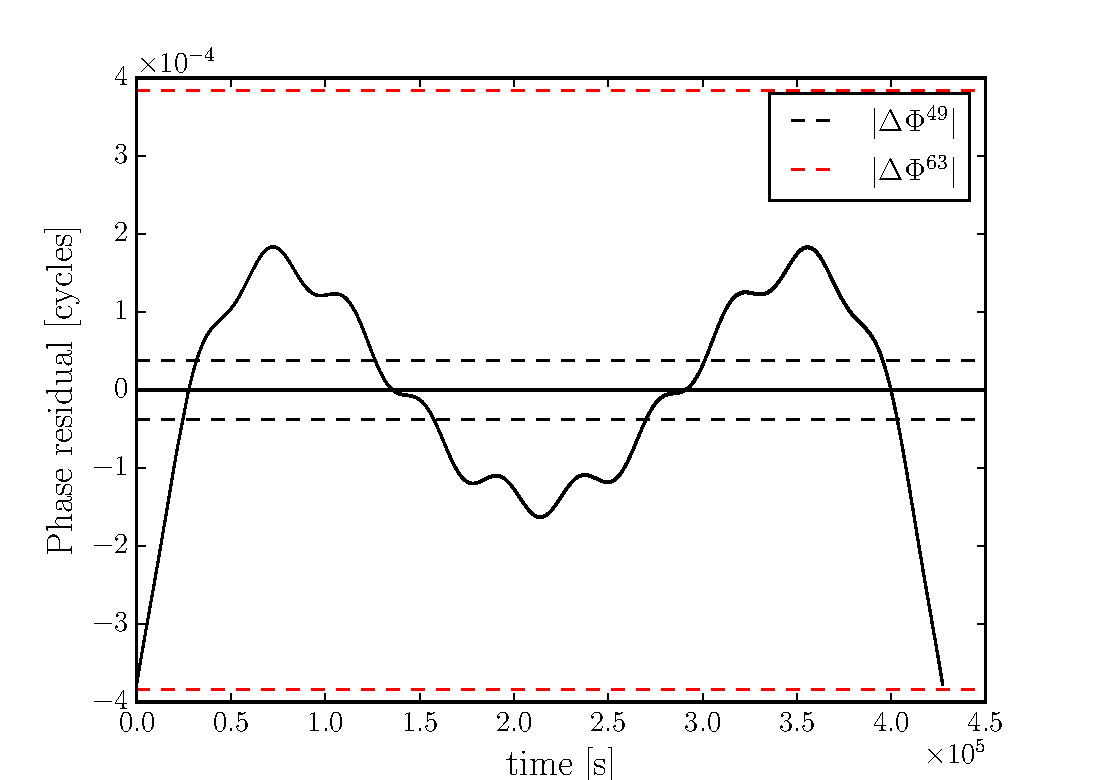
\includegraphics[width=0.5\textwidth]{NoSwitching.pdf}
}{%
    \caption{}
  \label{fig: no switching}
}
\capbtabbox{%
   \begin{tabular}{ccl}
\multicolumn{3}{c}{Simulation parameters} \\
\hline
$\omega_0$  &=& 15.0 rad/s\\
$B_0$  &=& $ 2.683\times 10^{15} $ G \\
$\chi$  &=& 60.10$^{\circ}$ \\
$a_0$ &=& -4.46$^{\circ}$ \\
$\tilde{\theta}$ &= & 0.02$^{\circ}$ \\
$\mathcal{A}_{\mathrm{EM}}$ &= & $31.0$
\end{tabular}
    
}{%
  \caption{}%
  \label{tab: NoSwitching properties}
}
\end{floatrow}
\end{figure}


We will now setup a simulation of this `minimal precession` NS, and then 
manually switch the torque. We choose a NS where the EM torque amplification
given in equation \eqref{eqn: Jones 75} is important.

\FloatBarrier
\subsection{Switching without the anomalous torque}
We now consider manually switching the spindown torque halfway though the simulation.
That is we set
\begin{align}
    t_{\mathrm{switch}} = \frac{\To}{2}, &&& \Ss = 0.4, &&& \Sa = 0.0,
\end{align}
such that halfway though the simulation the spindown torque is reduced by a
fraction $0.4$ while the anomalous torque remains unaffected. 

In figure \ref{fig: switching without anom} we plot the phase residuals from
this simulation. In the top plot is the residual as calculated over the entire
observation period. We find a single periodic variation with significantly
larger variation than any of the precession features. This is a direct result
of the switching only% as discussed in section \ref{sec: Lyne two state}:
the
effect of precession is entirely swamped by the switching. For this reason in
the lower plot we calculate two residuals: the first is calculated
in the region $[0, t_{\mathrm{switch}}]$ and the second in $[t_{\mathrm{switch}}, \To]$.
Because the switch does not occur in either of these periods we can resolve the
free precession during each period.

\begin{figure}[htb]
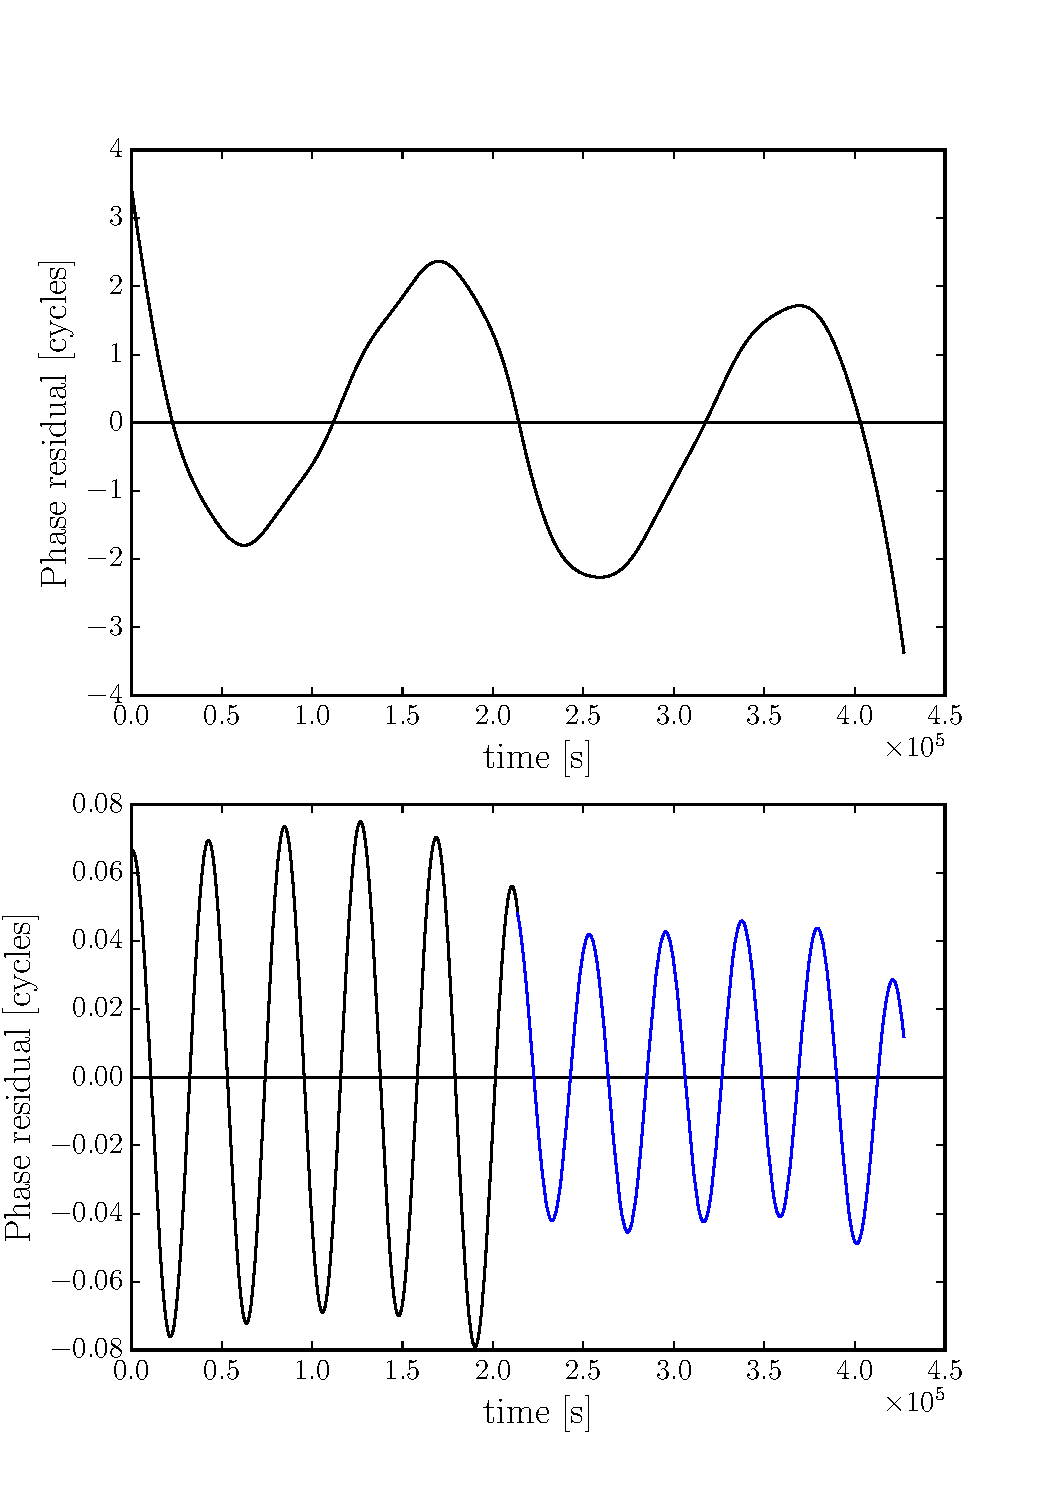
\includegraphics[width=.5\textwidth]{SwitchingWithoutAnomTorque}
\caption{}
\label{fig: switching without anom}
\end{figure}

The simulations begin in the minimal precession state where the spin-vector
is aligned with the effective body frame axis such that the wobble angle is given
by equation \eqref{eqn: spindown wobble angle}. After the switch, the wobble
angle is smaller by a factor $\Ss$ and as a result we see the precession is
reduced by this fraction.


\FloatBarrier
\subsection{Switching with the anomalous torque}
We now consider manually switching both the spindown and anomalous torque
halfway though the simulation.  That is we set
\begin{align}
    t_{\mathrm{switch}} = \frac{\To}{2}, &&& \Ss = \Sa = 0.01
\end{align}

In a similar fashion to figure \ref{fig: switching without anom} we show first
the total residual in the top plot of figure \ref{fig: switching with anom}, and
then the individual residuals in the lower plot.

In this simulation we have used a significantly smaller switching fraction 
than when switching without the anomalous torque. This is because the effect 
on the phase residuals when calculated in the two regions is significantly
stronger. This is because we begin with a `minimal precession' state, where
$\theta = \beta$ and the precession results from effect of the spin-down torque.
Then, when we switching off a fraction of the anomalous torque we have modified
the effective body frame and hence the angle $\beta$. This generates a significantly
larger wobble angle producing a significant increase in the phase residuals
fitted in the post-switch period. The effect is not observable when fitting
to the entire simulation period since the switching event remains dominant.

\begin{figure}[htb]
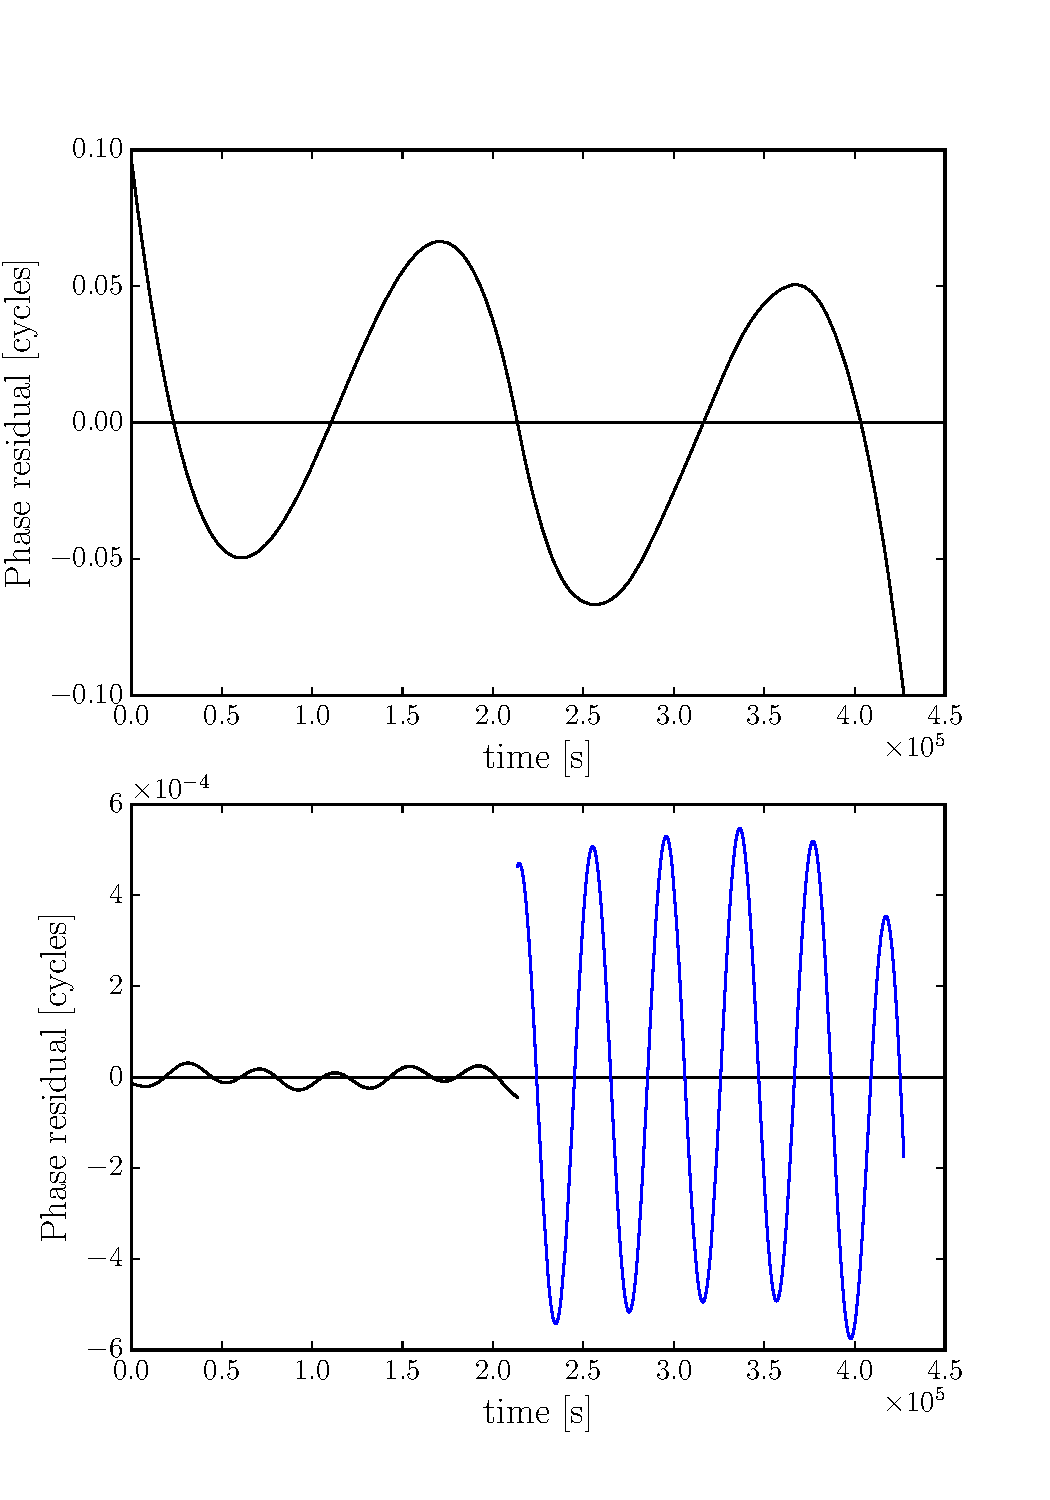
\includegraphics[width=.5\textwidth]{SwitchingWithAnomTorque}
\caption{}
\label{fig: switching with anom}
\end{figure}

\subsubsection{Calculating the new wobble angle after a switch}
We now calculate the change in wobble angle and hence phase-residual variations
after switching a fraction of the anomalous torque.
In our model the strength of the torque is parameterised
by $\epsA$, related to the surface magnetic field strength by 
\begin{align}
    \epsA = \frac{R^{5}}{4I_{0} c^{2}} B_{0}^{2}.
\end{align}
Rearranging equation (1.4.8) of my transfer thesis we can then write the 
spindown as 
\begin{align}
    \dot{\omega}_{0} & = -\frac{B_{0}^{2}R^{6} \sin^{2}(\alpha) \omega_{0}^{3}}{6 I_{0} c^{3}} \\
    & = - \frac{2 R \epsA \sin^{2}(\alpha) \omega_{0}^{3}}{3 c},
\end{align}
where $\alpha$ is the angle between the spin-vector and magnetic dipole. Since
we expect these to be misaligned in order to observe pulsations, we can take
$\sin^{2}\alpha \approx 1$.
Taking the spin frequency as a fixed value yeilds an estimate for the
spin-down frequency
\begin{equation}
    \fdot = - \frac{R\omega_{0}^{3}}{3\pi c}\epsA.
    \label{eqn: spin-down of epsA}
\end{equation}

In the two-state switching model, the spin-down value was observed to change
by a fraction $\upsilon$ such that
\begin{equation}
    \fdot \rightarrow \fdot' = (1-\upsilon)\fdot,
\end{equation}
then from equation \eqref{eqn: spin-down of epsA} 
\begin{equation}
    \epsA \rightarrow \epsA' = (1-\upsilon)\epsA.
\end{equation}

The two-state switching changes the value of $\epsA$ and so has a knock-on 
effect on the effective body frame. A non-precessing NS at an
angle $\beta(\epsI, \epsA, \chi)$ will, after a torque switch by a fractional
amount $\upsilon$, no longer be aligned with the body frame axis. This is 
because the effective body frame will have shifted to 
$\beta' = \beta(\epsI, \upsilon\epsA, \chi)$. As a result, we should expect the
previously non-precessing NS to begin precessing after a torque switching event. 

The NS will precess at the usual precession frequency in a cone  of half-angle
\begin{equation}
    \Delta\beta(\epsI, \epsA, \chi, \upsilon)=|\beta - \beta'|,
\end{equation}
about the new effective body-frame axis.  The expression for $\Delta \beta$ is
not easily amenable to manipulation, but can easily be explored graphically.
This is done in figure \ref{fig: DeltaBetaPlot} for several choices of
$\upsilon$. This illustrates that the precession angle can be as much as a few
degrees although it tends to zero in the limit $\epsI \gg \epsA$.

\begin{figure}[htb]
    \centering
    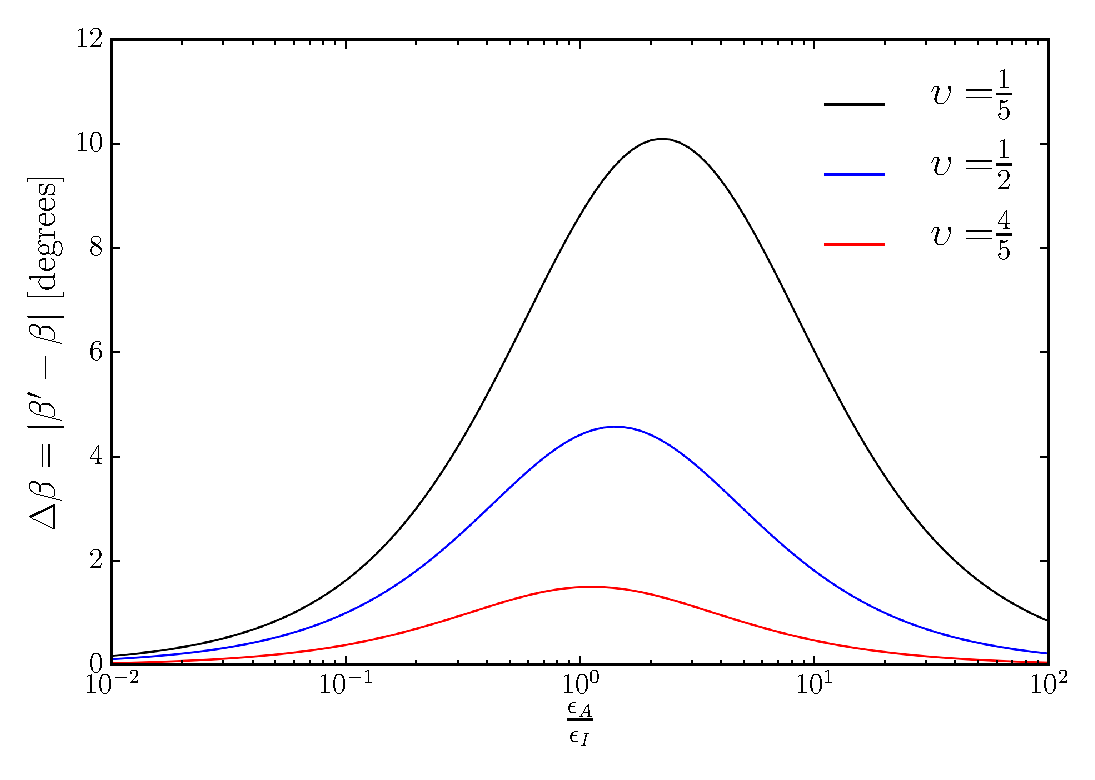
\includegraphics[width=0.5\textwidth]{DeltaBetaPlot}
    \caption{Illustrating the magnitude of the precession angle after switching
        due to the new rotation of the effect body frame. We plot the half-angle
        ($\Delta\beta$) of the precession cone as a function of the ratio
    $\epsA/\epsI$. Typically we expect real stars to have $\epsA < \epsI$.}
    \label{fig: DeltaBetaPlot}
\end{figure}

Since it is hard to gauge the significance of this we will apply it to the
PSR B1828-11; a pulsar which demonstrated evidence for precession \citet{Stairs2000}
and has since been reinterpreted as two-state switching \citep{Lyne2010}. This
has a frequency of $\f = 2.47$~Hz, a spin-down $\fdot=-3.65\times10^{-13}$~Hz/s, switches are
observed to occur every $T\approx 1.4$ yrs, and the spindown changes by $\upsilon = 0.71$.

We are unable to directly calculate $\Delta\beta$ from this information, since
we do now know $\epsI$ or $\chi$. Nevertheless, we can at least find the maximum
allowed value found when $\chi \ll 1$ and $\epsI \sim \epsA$. This has not 
been found exactly although it could easily be done by maximising the function 
numerically. Approximately the maximum allowed angle is $\Delta\beta \sim 45^{\circ}$.

We can now attempt to quantify the effect this may have on the timing residuals.
Precession, as shown by \citet{Jones2001}, will produce a sinusoidal variation
in the residual with a magnitude given by 
\begin{equation}
    \Delta\Phi_{\mathrm{FP}} \sim \pi \cot(\chi) \theta.
\end{equation}
This precession will be damped by other processes, but in the immediate aftermath
of a switch, may be detectable. 

However, when considering the residual which includes a switch we must also
take into acount the effect this will have. This was considered in section (6.6)
of my transfer thesis. Here we present the result that, the maximal size of phase-residuals
assuming several switched occur during an observation is given by 
\begin{equation}
    \Delta\Phi_{\mathrm{TS}} \sim \frac{\pi}{16} \upsilon \fdot  T^{2},
\end{equation}
Where $T$ is the switching period

For PSR B1828-11 then we can directly compute the magnitude of variations in
the timing residual:
\begin{align}
    \Delta t_{\mathrm{TS}}^{\mathrm{B1828-11}} \approx 70\mathrm{~ms}
\end{align}
This is considerably larger than the result from \citet{Lyne2010} who measured a 
peak to peak residual of 94 ms.





